
\begin{figure*}[t]
\centering
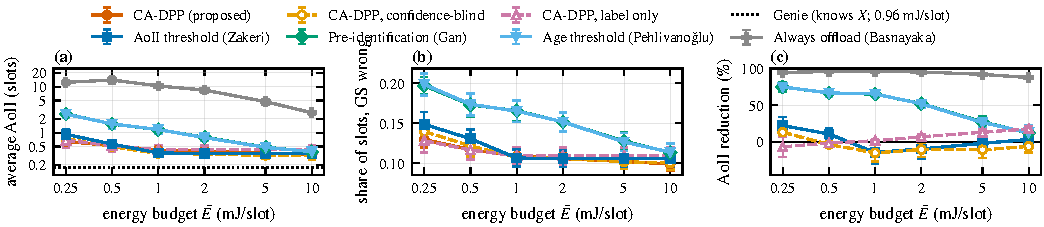
\includegraphics[width=\textwidth]{figures/fig_budget.pdf}
\caption{Energy budget sweep, $20$ held-out runs per point, with $95\%$ confidence intervals. (a) Average AoII. (b) Fraction of slots in which the GS is wrong. (c) AoII reduction by CA-DPP relative to each policy (paired intervals); negative values favor the other policy.}
\label{fig:budget}
\end{figure*}

\begin{figure*}[t]
\centering
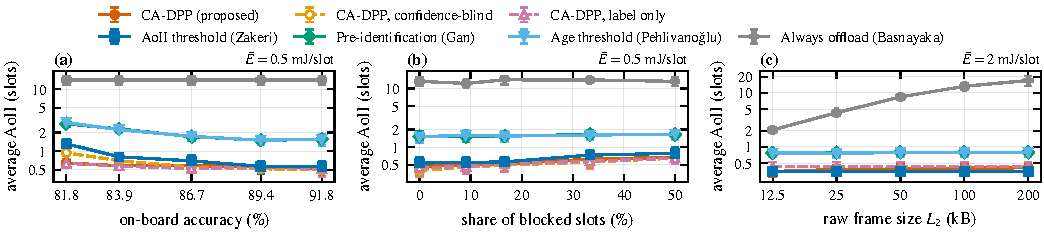
\includegraphics[width=\textwidth]{figures/fig_sensitivity.pdf}
\caption{Sensitivity ($20$ runs per point): (a) on-board accuracy and (b) share of blocked slots, $\rho_{\rm b}/(\rho_{\rm b}+\rho_{\rm u})$, at $\bar E=0.5$; (c) raw frame size at $\bar E=2$\,mJ/slot.}
\label{fig:sens}
\end{figure*}

\subsection{Data, Classifiers and Scenario}
We build traces from the hand-labeled part of Sen1Floods11~\cite{bonafilia2020sen1floods11}: 446 Sentinel-2 chips of $512\times512$ pixels at $10$\,m from eleven flood events, with official train, validation and test splits. A $64\times64$-pixel footprint scans each chip along a serpentine path with a stride of $32$ pixels, one footprint per slot, and is labeled flooded if at least $10\%$ of its labeled pixels are water. Footprints with less than $80\%$ labeled pixels are skipped, which leaves $46{,}774$, $16{,}612$ and $16{,}811$ slots in the three splits. Consecutive footprints overlap, so the state sequence is strongly correlated; on the training split $p_0=0.039$ and $p_1=0.166$. We use this Sentinel-2 imagery as a proxy for the UAV's downward view.

The on-board model is a logistic regression on the $8\times8$ average-pooled blue, green, red and near-infrared bands (257 parameters). The ground model is a gradient-boosted tree ensemble (300 trees) on 77 statistics of all 13 bands and two water indices. Both are trained on the training split and calibrated by isotonic regression on the validation split. To vary the on-board quality, we add Gaussian noise of $2$, $4$, $6$ and $8$ times the per-band standard deviation to its input and recalibrate. On the $174$ validation and test chips ($33{,}423$ slots, $20.5\%$ flooded), the five on-board variants are correct on $91.8\%$, $89.4\%$, $86.7\%$, $83.9\%$ and $81.8\%$ of the slots, and the ground model on $97.6\%$. Noise makes the on-board errors lopsided: the noisiest variant labels $7\%$ of the test slots as flooded, against $21\%$ in truth.

The UAV flies at $100$\,m on a circle of radius $1.3$\,km centered $1.5$\,km from the GS, so its distance to the GS ranges from $0.2$ to $2.8$\,km over one orbit of $400$ slots ($\tau=0.5$\,s). The link uses $2.4$\,GHz, $W=1$\,MHz, $20$\,dBm, a $7$\,dB noise figure and the urban parameters of~\cite{alhourani2014lap}. Blockage has $\rho_{\rm b}=0.02$ and $\rho_{\rm u}=0.1$, so $17\%$ of the slots are blocked, for $10$ slots on average. A label is $32$\,B and a raw frame $50$\,kB unless stated otherwise, with $\tau_{\max}=0.4$\,s, $P_{\rm r}=1$\,W and $E_{\rm o}=20$\,mJ. A label then costs about $20$\,mJ, while a raw upload costs $58$ to $420$\,mJ and succeeds with probability $0.99$ to $0.25$, depending on the distance. We use $\Delta_{\max}=300$.

\subsection{Baselines and Evaluation Protocol}
All baselines observe the same labels, confidences and link state as CA-DPP and stay within the budget through a token bucket with an initial credit of $0.5$\,J; when a raw upload does not fit, they send the label if they can. \begin{itemize}
\item AoII threshold, after~\cite{zakeri2023aoiieh}: the source model there has no classifier, so the UAV treats its label as the observed state and sends it once it has disagreed with the GS for $k\in\{1,2,3,5\}$ consecutive slots.
\item Pre-identification, after~\cite{gan2025taoi}: the UAV reports every label and uploads the frames labeled flooded for re-identification by the ground model.
\item Age threshold, after~\cite{pehlivanoglu2026orbit}: once $A\in\{1,3,10\}$ slots have passed since the last delivery, the UAV uploads raw data if $q_2(g)\ge q^\star\in\{0.5,0.9\}$ (or never) and sends the label otherwise.
\item Always offload, after~\cite{basnayaka2025aomi}: the UAV uploads the frame once $N\in\{1,2,5,10,50\}$ slots pass without a delivery.
\end{itemize}
Two ablations isolate parts of CA-DPP. The confidence-blind version replaces the confidence by the precision of the label value on tuning data, so its belief uses the class prior but ignores how sure the classifier is about each frame. The label-only version never uploads. A genie that knows $X(t)$ and sends an error-free update when the GS is wrong gives a floor.

Chips from the same flood event look alike, so results from a single tuning/test split depend strongly on which chips fall in each set. We therefore use $5$-fold cross-validation over the $174$ validation and test chips. For each fold, every parameter is chosen on the other four folds: $V$ (four values per budget, from $10^{-3}$ to $10$) and the belief ($\nu\in\{0.25,0.5\}$ with the class prior, or the symmetric update) for CA-DPP and its ablations, and the thresholds for the baselines. The same four folds give $\ee_{\rm g}(c)$, estimated in seven confidence bins, and the label precisions. We keep the parameter with the lowest AoII among those whose energy stays within $5\%$ of the budget, and run it four times on the held-out fold, each run visiting the chips four times in random order with fresh fading and blockage. This gives $20$ held-out runs per policy and setting. Runs with the same index share all random numbers, so we report paired $95\%$ confidence intervals of the relative change, paired $t$-tests and the number of folds won by CA-DPP.

\subsection{AoII Under an Energy Budget}
Against the pre-identification and age-threshold policies, CA-DPP lowers the AoII by $75\%$ at $0.25$\,mJ/slot, $52\%$ at $2$\,mJ/slot and $12\%$ at $10$\,mJ/slot (Fig.~\ref{fig:budget}, Table~\ref{tab:results}), in every fold up to $5$\,mJ/slot ($p<10^{-5}$). The first policy spends most of its energy on labels that confirm what the GS already believes, which Proposition~\ref{prop:confirm} shows to be worthless. The second reacts to the time since the last delivery, which says little about whether the GS is wrong. Offloading every update is an order of magnitude worse, since a raw frame costs $3$ to $21$ labels.

Against the AoII-threshold policy, results depend on the budget. At $0.25$\,mJ/slot, where the UAV can afford a label in about one slot in $100$, CA-DPP lowers the AoII by $22\%\pm12\%$ ($p=0.002$, four folds of five), and the $99$th AoII percentile drops from $19.2$ to $12.3$ slots. At $0.5$\,mJ/slot the reduction is $11\%\pm7\%$ and not significant ($p=0.10$). From $1$\,mJ/slot on, the threshold policy with $k=1$ reports every disagreement for about $0.84$\,mJ/slot and matches CA-DPP; the differences range from $-3\%$ to $+14\%$ with $p\ge0.09$. With cheap labels, the next frame corrects a wrong label, which the one-step gain of Lemma~\ref{lem:onestep} ignores; a discounted look-ahead did not help.

At $0.25$\,mJ/slot the per-frame confidence matters, and the confidence-blind version has a $15\%$ higher AoII ($p=0.001$). From $1$\,mJ/slot on, the confidence-blind version is $6\%$ to $15\%$ better than CA-DPP, significantly only at $1$\,mJ/slot ($p=0.02$). With this classifier, with ample energy, the precision of each label value gives the belief most of what it needs. Raw uploads pay off at larger budgets. Without them the AoII stays at $0.43$ from $1$\,mJ/slot on, while CA-DPP reaches $0.39$ at $2$\,mJ/slot and $0.34$ at $10$\,mJ/slot ($p\le0.001$). The genie reaches $0.171$ with $0.96$\,mJ/slot; most of the gap comes from not observing $X(t)$.

\subsection{Weak Classifiers, Blockage and Payload}
Fig.~\ref{fig:sens}(a) lowers the on-board accuracy at $0.5$\,mJ/slot. The AoII of CA-DPP grows only from $0.53$ to $0.64$ as the accuracy drops from $91.8\%$ to $81.8\%$, while that of the threshold policy grows from $0.56$ to $1.31$ and that of the confidence-blind version from $0.50$ to $0.94$. With the two noisiest models, CA-DPP is $27\%$ and $49\%$ better than the threshold policy and $14\%$ and $28\%$ better than the confidence-blind version, in all five folds ($p\le0.002$). With the two most accurate models the three policies are within the run-to-run spread. Per-frame confidence therefore pays off when the classifier is weak and its errors are lopsided, as is likely for a small on-board model.

As the share of blocked slots grows from $0$ to $50\%$ (Fig.~\ref{fig:sens}(b)), all policies lose ground and their order is unchanged. CA-DPP stays $9\%$ to $15\%$ below the threshold policy ($0.009\le p\le0.1$). The confidence-blind and label-only versions are $1.5\%$ to $11\%$ below CA-DPP, so at $0.5$\,mJ/slot raw uploads cost slightly more than they return. Fig.~\ref{fig:sens}(c) varies the raw frame size at $2$\,mJ/slot. With $12.5$\,kB frames CA-DPP is $15\%$ better than the label-only version and matches the threshold policy; with $200$\,kB frames the advantage over label-only shrinks to $3.5\%$, because the policy uploads less often as uploads get more expensive, without retuning.

\begin{figure}[t]
\centering
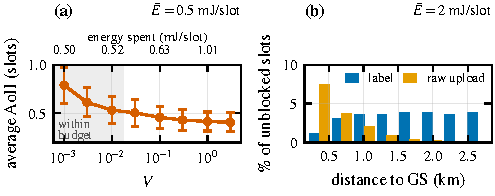
\includegraphics[width=\columnwidth]{figures/fig_V_mix.pdf}
\caption{(a) AoII of CA-DPP vs.\ $V$ at $\bar E=0.5$\,mJ/slot (top axis: energy spent; shaded: within $4\%$ of the budget). (b) Share of unblocked slots with a label or raw upload vs.\ distance to the GS, $\bar E=2$\,mJ/slot.}
\label{fig:Vmix}
\end{figure}

In Fig.~\ref{fig:Vmix}(a), at $0.5$\,mJ/slot, raising $V$ from $10^{-3}$ to $3$ lowers the AoII from $0.79$ to $0.41$, but the virtual queue builds up more slowly, and over a run of about $27{,}000$ slots the energy spent rises from $0.50$ to $1.51$\,mJ/slot. Values of $V$ up to $10^{-2}$ stay within $4\%$ of the budget. In Fig.~\ref{fig:Vmix}(b), at $2$\,mJ/slot and within $850$\,m of the GS, where uploads are cheap and reliable, CA-DPP uploads in $5.9\%$ of the unblocked slots and labels in $2.0\%$. Beyond $2.15$\,km it uploads in $0.1\%$ and labels in $3.8\%$.
